\section{Methodology}\label{sec:methods}

\subsection{Time Stepping Scheme}\label{sec:time-step-scheme}

The use of block-wise traversal has proven to increase performance by a large magnitude. 
% An \gls{lts} scheme should not interfere with this, but take advantage of it:
% therefore, an implementation of \gls{lts} in \gls{hms} required 
Therefore, it must be preserved when an \gls{lts} scheme is applied to \gls{hms}. This requires
the development of a novel time stepping scheme, which operates on blocks rather than individual cells.

\phantomsection\label{fix:flux-cost-share}
Benchmark cases have shown that flux computations account for up to 86\% 
of the program's runtime.
For that reason, the proposed \gls{lts} scheme for \gls{hms} focuses on reducing flux computations by adapting the \gls{frozen-flux-LTS} approach.
However, partly to maintain block-wise traversal, a few changes are necessary:
(i) The time step is uniform throughout the block. It is calculated for each cell and the block-wise minimum is set as its allowable time step $\Delta t_b$.
(ii) Instead of determining how many times the fluxes can be reused, a block flux expiry time is introduced on the base of the block's allowable time step in \autoref{eq:expiry-time}.
Accordingly, the scheme is named \gls{frozen-block-LTS}.
\begin{equation}
  \label{eq:expiry-time}
  t_{\text{expiry}, \, b} = t + \Delta t_b
\end{equation}

% This way, both \gls{simd} and \gls{mimd} parallel processing remain unchanged.

\begin{algorithm} [b]
  % alg1
  \caption{Parallelized time loop including block-wise traversal}
  \label{alg:bi_loop}
  \begin{algorithmic}[1]
    \small

    \State $t = t_0$ \Comment{get $t_0, t_{\text{end}}$ from \texttt{.ini} file}
    \State \Call{init\_persistent\_solver\_threads}{ }
    \State \textsc{bfm} = \Call{BlockFluxMemory}{ }

    \While{$t < t_{\text{end}}$}
      \ForAll{block $b$} \Comment{thread-parallel block-wise traversal}
        \\ {\color{white}} \; \;
        \Call{compute\_block}{$b$}
      \EndFor
      \State $t = t + \Delta t$ \Comment{proceed to next time index}
      \State $\Delta t = \min(\Delta t_{b})$ \Comment{set next global time step}
    \EndWhile
  \end{algorithmic}
\end{algorithm}

Upon start of the program, runtime-persistent objects are initialized, e.g., a user-defined number of persistent solver threads and a \gls{bfm} object for storing frozen block fluxes.
Details on the latter can be found in \autoref{sec:memory-structure}.
Subsequently, the time loop is started: each %epoch
time $t_n$, a loop traverses the domain on all solver threads in parallel: 
Each thread is assigned a set of blocks, which it processes one by one, by calling \textsc{compute\_block} (\autoref{alg:compute_block}) to advance its state to the next time $t_{n+1}$.
This includes the computation of fluxes, state variables and the allowable time step.
Once all blocks have been updated, the time is progressed: $t_{n+1} = t_{n} + \Delta t$. 
The next global time step is drawn from the minimum allowable time step $\Delta t = \min (\Delta t_b)$, ending the current time loop iteration.
\autoref{alg:bi_loop} sketches the described time loop in pseudocode.
\phantomsection\label{fix:conditional-statments}As a side note, at each time $t_n$, the program needs to decide just once for each block, instead of once per cell, whether to perform a full or scalar computation.
This leads to a reduced number of conditional statements,  which may reduce branching operations.

The time loop calls a function used to advance blocks: \textsc{compute\_block} (\autoref{alg:compute_block}).
This function is used to decide whether to carry out a full or scalar computation on the block fluxes based on expiry time. 
It delegates the actual block update to \textsc{compute\_block\_full} (\autoref{alg:compute_block_full}) and \textsc{compute\_block\_scalar} (\autoref{alg:compute_block_scalar}).
Criterion \ref{eq:frozen-block-criterion} decides on the type of computation.
\begin{equation}
  \label{eq:frozen-block-criterion}
  \text{action for block } b = 
  \left\{
    \begin{array}{ll}
      \text{full computation}, & \text{if } t_{\text{expiry}, \, b} \leq t + \Delta t \\
      \text{scalar computation}, & \text{otherwise}
    \end{array}
  \right.
\end{equation}

To automatically initiate a full flux computation at the beginning of the time loop, it is recommended to initialize expiry time to the lower numeric limit of the according datatype.

\begin{algorithm} [htb]
  % alg2
  \caption{Wrapper function for deducing whether to perform full or scalar computation}
  \label{alg:compute_block}
  \begin{algorithmic}[1]
    \small

    \Function{compute\_block}{$b$}
      \If{
        % \Call{bfm.block\_fluxes}{$b$}.expiryTime $< t + \Delta t$
        $t_{\text{expiry}, \, b} < t + \Delta t$
      }
      \State \Call{compute\_block\_full}{$b$}
      \Else
      \State \Call{compute\_block\_scalar}{$b$}
      \EndIf
    \EndFunction
  \end{algorithmic}
\end{algorithm}

It is necessary for a reuse of precomputed fluxes to save these in a way accessible for all solver threads. This is solved by the \gls{bfm}, which is introduced below in \autoref{sec:memory-structure}. 

A full block update consists of numerous steps, which have been grouped once more into multiple functions, which perform tasks in the given sequence:
\begin{enumerate}
  \item Initialize solver thread buffers for state variables with previous or, if time is $t_0$,  initial values
  \item Compute fluxes $\Delta \mathbf{q}_b$ using the flux term in \autoref{eq:disc-cl} and \gls{tvd} or first-order reconstruction
  \item Optionally, add mass sources and sinks to the storage buffer $\mathbf{q}_b$ 
  \item Optionally, apply friction source term to the fluxes $\Delta \mathbf{q}_b$
  \item Add fluxes to storage $\mathbf{q}_b = \mathbf{q}_b + \Delta \mathbf{q}_b$
  \item Compute new values for all state variables based on storage
  \item Compute allowable time step $\Delta t_b$  using \autoref{eq:cfl-time-step}
  \item De-scale fluxes by removing the current global time step and store them in \gls{bfm} for reuse
  \item Calculate $t_{\text{expiry}, \, b}$ and store it in \gls{bfm}
\end{enumerate}

\autoref{alg:compute_block_full} presents this sequence in the function \textsc{compute\_block\_full}.

\begin{algorithm} [b]
  % alg3
  \caption{Full block update function}
  \label{alg:compute_block_full}
  \begin{algorithmic}[1]
    \small

    \Function{compute\_block\_full}{$b$}
    \State \Call{compute\_storage}{$b$} \Comment{initialize solver thread buffers}
    \State $\Delta \mathbf{q}_b =$ \Call{compute\_fluxes}{$b$} \Comment{full flux calculation}
    \State \Call{add\_mass\_sources}{$b$} \Comment{optional, based on settings}
    \State \Call{compute\_friction}{$b$} \Comment{optional, based on settings}
    \State $\mathbf{q}_b = \mathbf{q}_b + \Delta \mathbf{q}_b$ \Comment{compute new storage state}
    \State \Call{compute\_new\_state}{$b$}
    \State $\Delta t_{b} =$ \Call{compute\_next\_timestep}{$b$} \Comment{compute next allowable block time step}
    \State \Call{bfm.block\_fluxes}{$b$}.fluxes $= \Delta \mathbf{q}_b / \Delta t$
    % \Comment{save fluxes for reuse in \textsc{bfm}}
    \State \Call{bfm.block\_fluxes}{$b$}.expiryTime $= t + \Delta t_{b}$ 
    % \Comment{save expiry time in \textsc{bfm}}
    \EndFunction
  \end{algorithmic}
\end{algorithm}

% Owning to the fact that the actual functions for advancing the blocks primarily differ by full and scalar computation of the fluxes, the corresponding functions are quite similar, as shown in \autoref{alg:compute_block_scalar}.

The two variants of the block update sequence are very similar: their main difference is a full or scalar computation of the fluxes; thus, the corresponding functions are quite similar as well. The latter is shown in \autoref{alg:compute_block_scalar} and described below.

Solver thread buffers are initialized in the same way as in a full update. 
Subsequently, previously saved fluxes are retrieved from \gls{bfm} and scaled with the current time step $\Delta t$. This is the scalar computation, replacing the more complex full computation.
While mass sources and sinks are applied in the same way as before, friction terms are left out because they are already included in the precomputed fluxes.
Finally, storage and new state variables are updated as usual.
Time step and saved fluxes in \gls{bfm} are left untouched, since fluxes have not been recomputed fully; therefore the existing expiry time remains.

\begin{algorithm} [ht]
  \caption{Scalar block update function}
  \label{alg:compute_block_scalar}
  \begin{algorithmic}[1]
    \small

    \Function{compute\_block\_scalar}{$b$}
      \State \Call{compute\_storage}{$b$} \Comment{initialize solver thread buffers}
      \State $\Delta \mathbf{q}_b =$ \Call{bfm.block\_fluxes}{$b$}.fluxes $* \Delta t$ \Comment{scalar flux calculation}
      \State \Call{add\_mass\_sources}{$b$}
      \State $\mathbf{q}_b = \mathbf{q}_b + \Delta \mathbf{q}_b$ \Comment{calculate new storage state}
      \State \Call{compute\_new\_state}{$b$}
    \EndFunction
  \end{algorithmic}
\end{algorithm}

\FloatBarrier
% Each blocks fluxes (represented by solid arrows and rectangles) are computed based on their own \gls{cfl} criterion (full computation).
% If a blocks current fluxes expiry time is larger than $\Delta t$ (the latter indicated by the dotted horizontal lines), its fluxes are scaled to match this time step (indicated by the dashed arrows).
% If expiry time of previously saved fluxes is larger than $\Delta t$ 
% As a result, the number of full computations is reduced as fluxes stored in \gls{bfm}.

The \gls{frozen-block-LTS} scheme is characterized by a very flexible approach:
each block's fluxes can be used nearly until their expiry time, i.e., until the last point in time $t_n$ before reaching expiry time. 
This is illustrated in \autoref{fig:frozen-block-lts-scheme}, which depicts the scheme similarly to \autoref{fig:pow2-LTS} for a small uniform mesh with four blocks.
To simplify this example, each block's allowable time step remains constant.
% There appear to be heterogeneous propagation velocities, as local time steps vary greatly.
Block $b=0$ sets the global time step $\Delta t$, as it has the smallest local time step. 
In contrast, block $b=2$ features a very large local time step, enabling it to use its fluxes for four times.
Block $b=3$ has a local time step less than half the size of $b=2$ but more than double the size of $b=0$, leading to a single reuse of its fluxes. 
Finally, the local time step of $b=1$ is less than $2 \Delta t$, causing it to perform full computation for each global time step, as fluxes cannot be reused in that case.

Overlaps of flux validity periods exist in all blocks, except for the one with the smallest allowable time step, in this case block ($b=0$). 
This is due to the fact that a new full computation always needs to start at a point in time $t_n$, not at the expiry time of the previously computed fluxes.
Thus, blocks with local time steps below $2 \Delta t$ need to perform a full flux computation each time.

\autoref{fig:pow2-LTS} can also be used for comparing \gls{frozen-block-LTS} to \gls{pow2-LTS}: we can clearly see it is possible for two neighboring regions to have large differences in their time steps in \gls{frozen-block-LTS}.
In \gls{pow2-LTS}, it is not recommended for levels to differ by more than a factor of two between directly adjacent regions.
\phantomsection\label{fix:pow2-LTS-drawbacks}Additionally, using an exponential term to set allowable time steps causes large overlaps of the fluxes' validity periods. 
This behavior increases with large local time steps:
e.g., a cell with local step $\Delta t_i \approx 126 \Delta t$ is assigned the allowable step of $\Delta t_m = 64 \Delta t$. 
Besides, such a large time step is only admitted, if at least eight \gls{lts}-levels are permitted, which can cause instabilities, as literature indicates \autocite{hu2019, sanders2008}.

\begin{figure} [htbp]
  \centering

  \begin{subfigure}{0.8\textwidth}
    \centering
    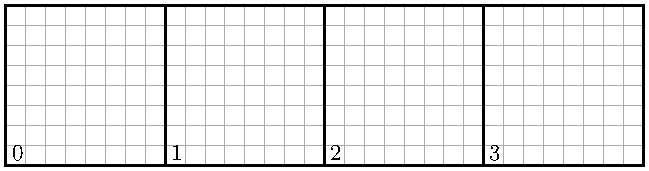
\includegraphics[width=0.7682\textwidth]{../typst/lts-scheme/lts_scheme-mesh.pdf}
    \caption[\Acrlong{lts} scheme mesh]{
      Uniform mesh with $32 \times 8$ cells and block size $8 \times 8$.
      Cell boundaries are shown in gray, while thick black lines indicate block boundaries.
    }\label{fig:frozen-block-lts-mesh}
  \end{subfigure}

  \vspace{0.5cm}

  \begin{subfigure}{0.8\textwidth}
    \centering
    \hspace{-1.05cm} % measured this to put b=1.5 in center
    \includegraphics[width=\textwidth]{../typst/lts-scheme/lts_scheme_overlap.pdf}
    \caption[\Acrlong{lts} scheme]{
      Illustrative \acrlong{frozen-block-LTS} block update procedure.
      Axes represent time and space (i.e., blocks).
      %epochs
      Points in time $t_n$, set apart by a constant $\Delta t$, appear as dotted horizontal lines.
      Blocks boundaries are shown as solid vertical lines; expiry time and therefore local time steps as solid horizontal lines.
      While solid upward arrows depict full block flux computations, dashed downward arrows symbolize scalar computations.
    }\label{fig:frozen-block-lts-scheme}

  \end{subfigure}
  % \caption[\Acrlong{frozen-block-LTS} scheme]{
  %   \Acrlong{frozen-block-LTS} scheme illustrated on a small fictional example.
  % }
  \caption{Illustration of the \acrlong{frozen-block-LTS}}
  \label{fig:frozen-block-lts}
\end{figure}

% \FloatBarrier

\subsection{Modifications to Frozen Block LTS} \label{sec:mods}
\subsubsection{Revised Criterion for Scalar Flux Computations}  \label{sec:criterion-mod}
The initial criterion for deciding on whether to perform full or scalar flux computations, \autoref{eq:frozen-block-criterion}, has shown to cause instabilities and a violation of mass conservation. Therefore, a modification is applied to counter this behavior. Criterion \ref{eq:frozen-block-criterion-mod} is adopted from \textcite{zhang1994a}, who developed it to work on similar stability problems of their \acrlong{frozen-flux-LTS} scheme.
\begin{equation}
  \label{eq:frozen-block-criterion-mod}
  \text{action for block } b = 
  \left\{
    \begin{array}{ll}
      \text{full computation}, & \text{if } t_{\text{expiry}, \, b} \leq t + 2 \Delta t\\
      \text{scalar computation}, & \text{otherwise}
    \end{array}
  \right.
\end{equation}

% This revision solved mass conservation, but causes larger overlaps and more frequent full flux computations. → Discussion/Outlook

\subsubsection{Neighbor Propagation}\label{sec:neighprop}
Initially, fluxes propagated poorly from high-velocity blocks to low-velocity neighbors, as they have larger local time steps. This, again, caused instabilities and loss of mass conservation.
An approach to synchronize heterogeneous regions is required to solve this problem.

Since the local time step is uniform throughout a block, it is deemed sufficient to implement a neighbor propagation technique, as described in \autoref{sec:LTS-smoothing}.
If a block is adjacent to one that requires a full computation based on \autoref{eq:frozen-block-criterion-mod}, it is forced to perform a full flux computation as well.
\autoref{alg:neighbor-propagation} shows a revision to \autoref{alg:compute_block}, including this neighbor propagation technique in combination with the improved criterion for scalar flux computations.
\begin{algorithm} [htbp]
  \caption{Revised function \textsc{compute\_block} including neighbor propagation and the improved criterion for scalar flux computations \autoref{eq:frozen-block-criterion-mod}}
  \label{alg:neighbor-propagation}
  \begin{algorithmic}[1]
    \small

    \Function{compute\_block}{$b$}

      \If{
        \Call{BFM.block\_fluxes}{$b$}.expiryTime $< t + 2 \Delta t$ 
        \\ {\color{white}} \; \; \textbf{or}
        \Call{BFM.neighbors\_require\_full\_computation}{$b$, $t + 2 \Delta t$}
      }
      \State \Call{compute\_block\_full}{$b$}
      \Else
      \State \Call{compute\_block\_scalar}{$b$}
      \EndIf

    \EndFunction
  \end{algorithmic}
\end{algorithm}

\FloatBarrier
\subsection{Block Flux Memory}\label{sec:memory-structure}

In the current implementation of \gls{hms}, only state variables are stored in memory, as all other variables are computed from the previous state. 
Other variables, like fluxes, are temporarily stored in solver thread buffers.
Thus, to enable reuse of fluxes, an additional memory structure is needed.
A two stage approach was chosen for this task:
Firstly, the implementation of a structure \texttt{BlockFluxes}, which stores fluxes and expiry time for each block;
secondly, the creation of a class \texttt{BlockFluxMemory}, which manages \texttt{BlockFluxes} objects and implements the concept of a \acrlong{bfm}. 
It stores a \texttt{std::vector} of \texttt{BlockFluxes} and various member variables which help to index the blocks. 
\texttt{BlockFluxMemory} provides access functions for \texttt{BlockFluxes} objects and all relevant member variables, as well as a function to determine whether a neighbor block requires a full computation to enable neighbor propagation.

Since \gls{hms} supports both first-order and \gls{tvd} reconstruction, the \acrlong{bfm} needs to adapt to either option's partitioning scheme.

\begin{figure}[!b]
  \centering
  \includegraphics[width=0.7\textwidth]{../typst/bfm-index/bfm-index-fo.pdf}
  \caption[\Acrlong{bfm}: Block map for first-order scheme]{
    \Acrlong{bfm}: Block map for the use with a first-order scheme.
    Cell boundaries are drawn as gray lines, whereas the block boundaries are depicted in black.
    The block index is shown in each block's bottom-left corner.
    Block size: $7 \times 7$ cells, mesh size: $37 \times 30$ cells.
  }
  \label{fig:bfm-index-fo}
\end{figure}

% Block partitioning for the first-order scheme is rather simple, as there are no boundary blocks. 
When using first-order reconstruction, the mesh is partitioned into blocks of fixed, user-specifiable sizes and smaller remainder blocks, as shown in \autoref{fig:bfm-index-fo}.
Starting from the bottom-left corner, the domain is filled with full blocks. 
Block size is not required to adapt to mesh size; thus, possible remaining cells are covered with smaller remainder blocks.

In contrast, block-wise traversal for the \gls{tvd} scheme requires a layer of blocks wrapping the mesh's boundary, having a fixed width of two cells.
This is due to the nature of second-order schemes, which take derivates of multiple cells' values around an edge into account to compute the fluxes over that edge.
Narrow blocks enable correct usage of the \gls{tvd} scheme at the domains boundaries.
A more complex partitioning scheme than for the first-order scheme results of this, as shown in \autoref{fig:bfm-index-tvd}.

\begin{figure}[!b]
  \centering
  \includegraphics[width=0.7\textwidth]{../typst/bfm-index/bfm-index-tvd.pdf}
  \caption[\Acrlong{bfm}: Block map for \acrshort{tvd} scheme]{
    \Acrlong{bfm}: Block map for the use with a \acrshort{tvd} scheme.
    Cell boundaries are drawn as gray lines, whereas the block boundaries are depicted in black.
    The block index is shown in each block's bottom-left corner.
    Block size: $7 \times 7$ cells, mesh size: $37 \times 30$ cells, boundary layer width: $2$ cells.
  }
  \label{fig:bfm-index-tvd}
\end{figure}

Currently, \gls{hms} identifies blocks by the coordinate of the cell in their bottom-left corner.
Thus, the \acrlong{bfm} needs to introduce an indexing mechanism according to both partitioning schemes for accessing \texttt{BlockFluxes} based block coordinates.
% , which is done by starting with inner blocks, including their remainders, followed by bottom, top, left and right boundary blocks, and finally corner blocks.
% To enable performant indexing, \gls{bfm} stores start index and number of blocks for each \texttt{BlockLocation}, which are assigned during initialization of a \gls{bfm} object and are accessed using the \texttt{blockIndex(\dots)} member function.
An additional \gls{2D} vector stores all block index numbers in a two-dimensional representation for efficiently retrieving adjacent blocks. 
% The location for each block in this 2D vector is stored in \texttt{BlockFluxes}.

The \gls{bfm} is instantiated at the start of each run of a \gls{hms} before the time loop starts.
Upon initialization, member variables for block indexing are populated, a \texttt{BlockFluxes} object for each block is constructed, and stored in a vector, at the position corresponding to its block index.
% Existing functions for computing blocks in \gls{hms} were adapted to utilize \gls{bfm} access functions for storing and reusing precomputed fluxes, as explained in \autoref{sec:time-step-scheme}.
% After finishing the time loop, a logger is used to output a summary for all blocks, which is used to generate a statistic as shown later in {fig:heatmap-dambreak}.

\FloatBarrier
\subsection{Test Cases and Metrics}
\label{sec:test-cases-metrics}

\subsubsection{1D Dam Break} \label{sec:case-dambreak}
To validate the proposed \gls{lts} model, the \gls{1D} schematic dam break case is used,
as an analytical solution for this case is available for comparison.
It consists of a domain of $\SI{20}{\meter} \times \SI{2}{\meter}$, discretized using $400 \times 40$ cells of $\SI{0.05}{\meter} \times \SI{0.05}{\meter}$ size, grouped into blocks of $8 \times 8$ cells.
Upstream and downstream boundaries are set to allow free outflow. 
% The two other boundaries do not allow that, to mimic the behavior of a \gls{1D} dam break.
The lateral boundaries act as frictionless walls to obtain a \gls{1D} flow pattern.
Two variants of this scenario are simulated:
(i) a wet case, in which the whole domain is covered in water, with a water depth of $d = \SI{4}{\meter}$ in the left and $d = \SI{1}{\meter}$ in the right half,
and (ii) a dry case, in which only the left half of the domain contains water, with $d = \SI{4}{\meter}$, whereas the right half is dry, i.e., $d = \SI{0}{\meter}$.
Flow velocity is set to $u=v=0$ in either case, 
and bed friction is not included.
The analytical solutions to these cases, used as a reference, are taken from \textcite{adelmann2022}.
Results are interpreted both visually and with the \gls{nse}, see \autoref{sec:metrics}, as a quantitative metric for accuracy.

As a base configuration for investigating the runtime reduction obtainable through \gls{lts}, a scaled-up variant of the wet dam break case with bed friction enabled is chosen.
Utilizing a fully wetted domain removes the consideration of load imbalances from the investigation, as \gls{hms} contains dry cell optimizations, which may otherwise introduce such effects.

For this base configuration, the domain consists of $2000 \times 2000$ cells of $d_x = d_y = \SI{1.0}{\meter}$, grouped into blocks of $64 \times 64$ cells; 
the Courant number is set to $\Cr = 0.3$ and the end time of the simulation to $t_{end} = \SI{0.6}{\second}$.

Multiple parameters are examined in terms of their impact on computational cost. 
These include domain, cell, and block sizes, the Courant number, water depth of the downstream region, and the simulated duration.
For domain, cell, and block sizes, downstream water depth, as well as the Courant number, a range of values both above and below the original configuration of $\Cr = 0.3$ are investigated.
For the simulated duration, the original value is used as a lower limit of the considered range.
Finally, the effects of disabling bed friction are examined, as well as of exchanging the scenario to a dry dam break with the same parameters as the base configuration.
For each variant, only a single parameter of the base configuration is modified, thus allowing to isolate their effects. 
All cases are run for each combination of first-order/\gls{tvd} reconstruction and global/local time stepping. 
To mitigate statistical variance, every configuration is run 25 times for each combination of reconstruction and time stepping schemes.

\subsubsection{Practical Case: Rainfall-Runoff in an Urban Area} \label{sec:case-moabit}
In order to assess the runtime reduction obtained with the \gls{frozen-block-LTS} in a practical application, a heavy precipitation event in an urban area in central Berlin, Germany, is simulated.
The domain covers $2048 \times \SI{2000}{\meter}$ with cells of $d_x = d_y = \SI{1.0}{\meter}$, grouped into blocks of $64 \times 64$ cells; 
the Courant number is set to $\Cr = 0.3$ and the end time of the simulation to $t_{end} = \SI{1200}{\second}$.
The precipitation data is taken from \textcite{fischer2024}.
For measuring accuracy in these cases, the \gls{sae} is used, see \autoref{sec:metrics}.

\subsubsection{Metrics} \label{sec:metrics}

\autoref{eq:nse} defines the \gls{nse} for some variable $\gamma$, with $\gamma_{\text{num}}$ as the numerical solution, 
the analytical or reference solution $\gamma_{\text{ref}}$,
and the mean value of the reference solution throughout time $\gamma_{\text{ref, mean}}$ \autocite{nash1970}:

\begin{equation}
  \label{eq:nse}
  \mathrm{NSE}(\gamma) = 1 - \frac{
      \sum_{t_0}^{t_{\max}} \left( \gamma^t_{\text{ref}} -\gamma^t_{\text{num}} \right)^2
    }{
      \sum_{t_0}^{t_{\max}} \left( \gamma^t_{\text{ref}} -\gamma_{\text{ref, mean}} \right)^2
    }
\end{equation}

\autoref{eq:sae} defines the \gls{sae} for some variable $\gamma$, with $\gamma_{\text{LTS}}$ and $\gamma_{\text{GTS}}$ as the numerical solutions obtained with \gls{lts} and \gls{gts}, respectively:

\begin{equation}
  \label{eq:sae}
  \mathrm{SAE}(\gamma) = \sum \abs*{\gamma_{\text{LTS}} - \gamma_{\text{GTS}}}
\end{equation}